\chapter{Spin 1/2}
The Hamiltonian for a single spin in a magnetic field $\mathbf B$ is
\begin{equation}
    H=-\mu\mathbf B \cdot \mathbf S
\end{equation} 
for spin $1/2$ we have using sigma matrices
\begin{equation}
    S=\frac{\hbar}{2}\left(\sigma_x,\sigma_y,\sigma_z\right) \equiv \frac{\hbar}{2}\left(\left(
\begin{array}{cc}
 0 & 1 \\
 1 & 0 \\
\end{array}
\right),\left(
\begin{array}{cc}
 0 & -i \\
 i & 0 \\
\end{array}
\right),\left(
\begin{array}{cc}
 1 & 0 \\
 0 & -1 \\
\end{array}
\right)\right)
\end{equation}

The coordinate system can be oriented such that $\mathbf B=(0,0,B_z)$ and eigenfunctions of the spin are thus in spherical coordinates $\theta,\phi$ and x-representation
\begin{align}
    u_1=\begin{pmatrix}
        \cos\frac{\theta}{2}e^{-i\phi}\\
        \sin\frac{\theta}{2}
    \end{pmatrix};\qquad
    u_2=\begin{pmatrix}
        -\sin\frac{\theta}{2}e^{-i\phi}\\
        \cos\frac{\theta}{2}
    \end{pmatrix}
\end{align}
For both of these states the Berry connection can be defined using \ref{eq:berryConnection}
\begin{equation}
   A^{(u_1)} = \begin{pmatrix}
    \braket{u_1| \der{u_1}{\theta}}\\
    \braket{u_1| \der{u_1}{\phi}}
   \end{pmatrix};\qquad 
   A^{(u_2)} = \begin{pmatrix}
    \braket{u_2| \der{u_2}{\theta}}\\
    \braket{u_2| \der{u_2}{\phi}}
   \end{pmatrix}
\end{equation}
and geometric tensor using \ref{eq:geometricTensor} we have
\begin{equation}
    \chi^{(u_k)}_{ij} = 
        \braket{\partial_i u_k|\partial_j u_k}-\braket{\partial_i u_k| u_k}\braket{u_k|\partial_j u_k} 
\end{equation}
implying
\begin{equation}
    \chi^{(u_1)} = \begin{pmatrix}
        \frac{1}{4}& \frac{i}{4}\sin\theta\\
        -\frac{i}{4}\sin\theta&\frac{\sin^2\theta}{4}
    \end{pmatrix};\quad 
    \chi^{(u_2)} = \begin{pmatrix}
        \frac{1}{4}& -\frac{i}{4}\sin\theta\\
        \frac{i}{4}\sin\theta&\frac{\sin^2\theta}{4}
    \end{pmatrix}.
\end{equation}
It's real part is according to \ref{eq:metrictensorREdefinition} the metric tensor
\begin{equation}
    g^{(u_1)} = g^{(u_2)} =\begin{pmatrix}
        \frac{1}{4}& 0\\
        0&\frac{\sin^2\theta}{4}
    \end{pmatrix}
\end{equation}
\textcolor{red}{For two state system, the metric tensor is always the same for both states. (just guessing now :).} Berry curvature can be easily calculated as minus imaginary part of the geometric tensor. 

\textcolor{blue}{
From the metric the Ricci curvature and Gaussian curvature are
\begin{align}
    R&=\begin{pmatrix}
        1&0\\
        0&\frac{1}{4}\sin^2\theta
    \end{pmatrix}\\
    K&=\frac{1}{8}(1+\sin^4\theta)
\end{align}
}

If the magnetic field is positive, $u_1$ is the ground state. The metric on $\M_0$ is then $g^{(u_1)}$ calculated above. During some arbitrary change of magnetic field whilst not measuring the state of the system, it can be transported from $\ket{\psi_i}\coloneqq \ket{u_1}$ to some new ground state by changing the magnetic field direction, as shown on fig. \ref{fig:blochArbitraryTransport}
\begin{figure}[h]
    \centering
    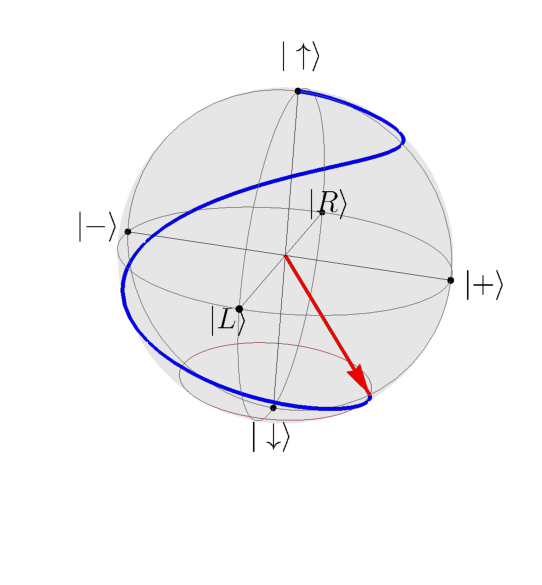
\includegraphics{../img/blochArbitraryTransport.pdf}
    \caption{Bloch sphere for the eigenstate $u_1$ with the initial direction of magnetic field $\mathbf B=(0,0,B_z)$ transported along $\gamma=\{(\phi,\sqrt{\phi})|\phi\in[0,2\pi]\}$ (blue). The final orientation of the magnetic field is marked red and the states on the Bloch sphere correspond to initial eigenstate.}
    \label{fig:blochArbitraryTransport}
\end{figure}

It's pedagogical to point out the correspondence to figure \ref{fig:manifoldCutIntuition}, where $\M_0=\cup_\llambda \{\ket{u_1}\}$,  $\M_1=\cup_\llambda \{\ket{u_2}\}$, $\ket{o(\llambda)}=u_1(\mathbf B=B(0,0))$ and $\ket{o(\tilde\llambda)}=u_1(\mathbf B=B(2\pi,\sqrt{2\pi}))$, written in spherical coordinates.


If the transport is made infinitesimally slow with respect to time $t$, after every step $\d \theta$ the eigensystem has to be calculated, and we find out that the system collapses into instantaneous $u_1(t)$ state of $\H(t)$, so the fidelity at any $\theta$ is $f_0(\theta)=1$ and $\d s^2(\theta)=1-f_0^2=0$. Opposite to the adiabatic transport would be the quantum quench, meaning the orientation of $\mathbf B$ is changed instantly resulting in a final state 
\begin{equation}
   \ket{f} = \alpha \ket{u_1} + \beta \ket{u_2}, \qquad\text{for } \frac{\alpha}{\beta}=e^{-i\phi}\tan\frac{\theta}{2},\quad \alpha^2+\beta^2=1.
\end{equation}
This yields probability of staying in the state $u_1$ after quench is $f_q=\braket{u_1|f}=\alpha$ and $s=1-\alpha$.

\section{Special case}
Assume again transport of $\ket{u_1}$ by rotating the magnetic field along the path $\gamma=\{(0,\theta)|\theta\in[0,\pi/2]\}$, as drawn on figure \ref{fig:blochPiHalfTransport}. The fidelity for infinitesimal speed is at every point on the path $f_0=1$ and for quantum quench $f_q=1/2$.

\textcolor{blue}{Now let's calculate the fidelity for some finite time transport. }
\begin{figure}[h]
    \centering
    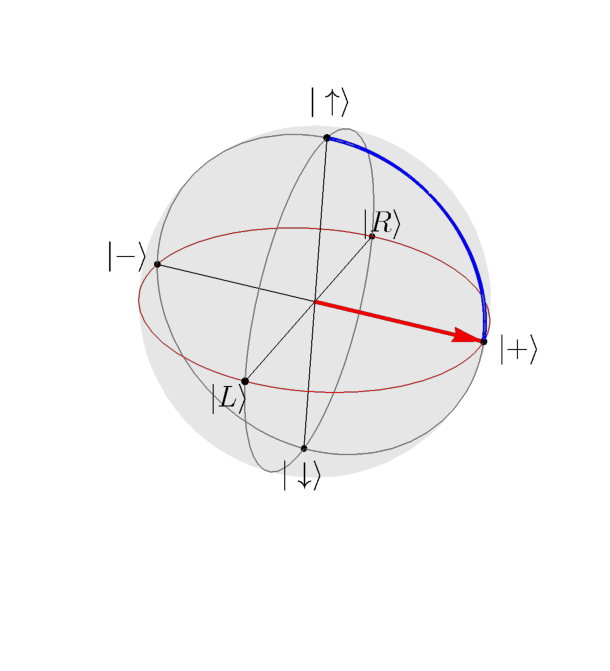
\includegraphics{../img/blochPiHalfTransport.pdf}
    \caption{Bloch sphere for the eigenstate $u_1$ with the initial direction of magnetic field $\mathbf B=(0,0,B_z)$ transported along $\gamma=\{(0,\theta)|\theta\in[0,\pi/2]\}$ (blue). The final orientation of the magnetic field is marked red and the states on the Bloch sphere correspond to initial eigenstate.}
    \label{fig:blochPiHalfTransport}
\end{figure}


